\subsection{Results}
\label{subsec:imagelocresults}

Again HOG features are used describe image patches. This time a more dense field
is required because from the image patches classified as \emph{image} the actual
images are to be extracted. For this purpose the page is divided into 10 by 20
blocks each with one cell. Optionally, features are concatenated to incorporate
more information from the region. This results in 9 by 19 concatenated
features: one feature, the features of the block to the right, to the bottom and
the right bottom are concatenated into one.

If the preprocessing step of the linear SVM is used, we need to be careful and
avoid over fitting by training the linear SVM on the same data as the structured
SVM is trained. Therefor, we used two stage validation learning (see figure
\ref{fig:twostage}). In two stage validation repeatedly, a different subset of
the training data is used to train the linear SVM. The resulting SVM assigns the
confidence score to rest of the training data in order to finally recreate the
whole training data, but now with confidence scores without the risk of
overfitting.
\todo{several SVMs and the confidence scores can be used?! Could only find:
\cite{duan2005best} which indicates exactly the opposite}

\begin{figure}
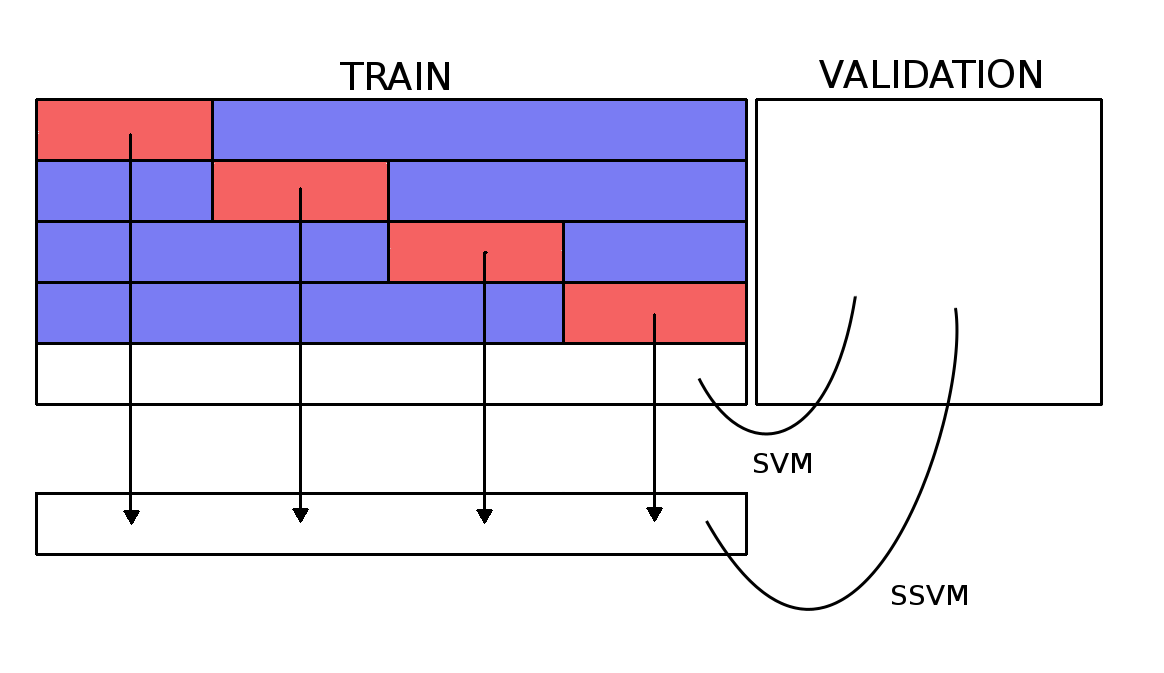
\includegraphics[width=.5\textwidth]{resources/twostage}
\label{fig:twostage}
\caption{Visualization of two-stage validation training to generate data for the
structured SVM}
\end{figure}

We experimented with 4 different settings: directly trained on the structured
SVM and pre-trained with the linear SVM, we then tested both options with the
concatenated features and with the regular features. The same division for the
train, validation and test set has been used as in section \ref{sec:pageclas}.
Tables \ref{tab:imagelocm} and \ref{tab:imagelocresults} show the results for
these settings. The `SVM Only' columns show the results of the
linear SVM for classifying single features. All scores are calculated per
feature. The true labels are based on the annotated data: whether their centre
is inside or outside a bounding box.

First, the results for the single HOG features in table \ref{tabl:imageloccm}.
The extremely low precision indicates that these single HOG features are not
indicative if an image patch belongs to an image or text. Presumably, this
large error propagates through to the pre-trained setting, resulting in a low
recall for image patches there as well. The directly trained SVM was able to
achieve much better results.

\begin{table}
\centering
% Extra colsep creates fancy lines
\begin{tabular}{@{\extracolsep{4pt}}l r r r r r r @{}}
\hline
& \multicolumn{2}{c}{\emph{SVM only}} & \multicolumn{2}{c}{\emph{Pre-trained}} & \multicolumn{2}{c}{\emph{Direct}}
\\\cline{2-3}\cline{4-5}\cline{6-7}
& \textbf{Image} & \textbf{Text} & \textbf{Image} & \textbf{Text} & \textbf{Image} & \textbf{Text} \\
%\textbf{Precision} & 0.099 & 0.973 & 0.271 & 0.979 & 0.271 & 0.979 \\
%\textbf{Recall} & 0.736 & 0.585 & 0.700 & 0.884 & 0.700 & 0.884 \\
%\textbf{F-score} & 0.174 & 0.730 & 0.391 & 0.929 & 0.391 & 0.929\\\hline
%%% NOOOOOO wrooonnggg!
\textbf{Precision} & 0.099 & 0.973 & 0.703 & 0.944 & 0.271 & 0.979 \\
\textbf{Recall}    & 0.736 & 0.585 & 0.040 & 0.999 & 0.700 & 0.884 \\
\textbf{F-score}   & 0.174 & 0.730 & 0.075 & 0.970 & 0.391 & 0.929\\\hline
\end{tabular}
\caption{Results for image localization with single features}
\label{tab:imageloccm}
\end{table}

Second, the results for the concatenated features in table
\ref{tab:imagelocresults}. The concatenated features seem to convey more
information about the image patch, as indicated by the rise in precision and
recall for the linear SVM. As a result, the score difference 
in the pre-trained and the directly trained experiments are small, but favor the
pre-trained setting slightly.

\begin{table}
\centering
\begin{tabular}{@{\extracolsep{4pt}}l r r r r r r @{}}
\hline
 & \multicolumn{2}{c}{\emph{SVM Only}}  & \multicolumn{2}{c}{\emph{Pre-trained}} & \multicolumn{2}{c}{\emph{Direct}} \\
 \cline{2-3} \cline{4-5} \cline{6-7}
  & \textbf{Image} & \textbf{Text} & \textbf{Image} & \textbf{Text} & \textbf{Image} & \textbf{Text} \\
\textbf{Precision} & 0.154 & 0.973 & 0.269 & 0.979 & 0.241 & 0.979 \\
\textbf{Recall} & 0.732 & 0.709 & 0.743 & 0.854 &  0.750 & 0.830 \\
\textbf{F-score} & 0.254 & 0.820 & 0.395 & 0.912 & 0.365 & 0.898 \\\hline
\end{tabular}
\caption{scores for image localization with concatenated features}
\label{tab:imagelocresults}
\end{table}

We can deduce that the CRF, solved by the structured SVM improves performance
significantly.


%\begin{table}
%\centering
%% Extra colsep creates fancy lines
%\begin{tabular}{@{\extracolsep{4pt}}l r r r r r r @{}}
%\hline
%& \multicolumn{2}{c}{\emph{SVM only}} & \multicolumn{2}{c}{\emph{Pre-trained}} & \multicolumn{2}{c}{\emph{Direct}}
%\\\cline{2-3}\cline{4-5}\cline{6-7}
%Real\textbackslash Predicted & \textbf{Image} & \textbf{Text} & \textbf{Image} & \textbf{Text} & \textbf{Image} & \textbf{Text} \\
%\textbf{Image} & 24160 & 8844 & 524523 & 58481 & 524759 & 58245 \\
%\textbf{Text} & 133044 & 324380 & 566567 & 5390857 & 577927 & 5379497 \\\hline
%\end{tabular}
%\caption{Confusion Matrix for image localization with concatenated features}
%\label{tab:imageloccm}
%\end{table}


%\begin{table}
%\centering
%% Extra colsep creates fancy lines
%\begin{tabular}{@{\extracolsep{4pt}}l r r r r r r @{}}
%\hline
%& \multicolumn{2}{c}{\emph{SVM only}} & \multicolumn{2}{c}{\emph{Pre-trained}} & \multicolumn{2}{c}{\emph{Direct}}
%\\\cline{2-3}\cline{4-5}\cline{6-7}
%Real\textbackslash Predicted & \textbf{Image} & \textbf{Text} & \textbf{Image} & \textbf{Text} & \textbf{Image} & \textbf{Text} \\
%\textbf{Image} & 24565 & 8800 &  523370 &  59995 & 523370 & 59995 \\
%\textbf{Text} & 224329 & 315906 &  562795 &  5477440 & 562795 & 5477440\\\hline
%\end{tabular}
%\caption{Confusion Matrix for image localization with concatenated features}
%\label{tab:imageloccm}
%\end{table}

%\todo{Explain results, mention that the difference between Pre-trained and
%not pre-trained is bigger with more discriminative features (2x2 HOG in stead of
%1)}

\todo{Visualisations of the results (if possible). Thomas mentioned showing some
pages with the classification as a colored overlay, or a map of the labels under
the page}
